\documentclass[
      aspectratio=169,
        12pt,
    ]{beamer}

% ------------------------------------ font
\usefonttheme[onlymath]{serif}
\usepackage[T1]{fontenc}
\usepackage{textcomp}
\usepackage[scale = 1.0]{tgheros} %Sans serif
\usepackage[scaled]{beramono}
\usepackage{luatexja-otf}
\usepackage[match, deluxe, expert, noto-otf]{luatexja-preset}
\renewcommand{\kanjifamilydefault}{\gtdefault}

% ------------------------------------ math packages
\usepackage{amsmath,amssymb}
\usepackage{siunitx}

% ------------------------------------ comment out package
\usepackage{comment}

% ------------------------------------ tables
\usepackage{longtable, booktabs, array}
\usepackage{threeparttable, threeparttablex, multirow}
\newcolumntype{d}{S[input-symbols = ()]}

% ------------------------------------ figures
\usepackage{graphics, graphicx}
\makeatletter
\def\maxwidth{\ifdim\Gin@nat@width>\linewidth\linewidth\else\Gin@nat@width\fi}
\def\maxheight{\ifdim\Gin@nat@height>\textheight\textheight\else\Gin@nat@height\fi}
\makeatother
% Scale images if necessary, so that they will not overflow the page
% margins by default, and it is still possible to overwrite the defaults
% using explicit options in \includegraphics[width, height, ...]{}
\setkeys{Gin}{width=\maxwidth,height=\maxheight,keepaspectratio}

\usepackage{tikz}
\usetikzlibrary{backgrounds}

% ------------------------------------ other packages (header-includes)

% ------------------------------------ Slide Designs
\definecolor{DarkBlue}{rgb}{0.05, 0.15, 0.35} 

\setbeamercolor{item}{fg=DarkBlue}
\setbeamercolor{title}{fg=DarkBlue}
\setbeamercolor{subtitle}{fg=DarkBlue}
\setbeamercolor{frametitle}{fg=DarkBlue}
\setbeamercolor{section title}{fg=white}

\renewcommand{\textbf}[1]{{\color{DarkBlue}\bfseries#1}}

\setbeamerfont{title}{size=\LARGE,series=\bfseries}
\setbeamerfont{subtitle}{size=\small,series=\bfseries}
\setbeamerfont{institute}{size=\scriptsize}
\setbeamerfont{date}{size=\scriptsize}
\setbeamerfont{section title}{size=\LARGE,series=\bfseries}
\setbeamerfont{frametitle}{size=\Large,series=\bfseries}

\setbeamertemplate{navigation symbols}{}
\setbeamertemplate{footline}[frame number]
\setbeamertemplate{itemize item}[circle]
\setbeamertemplate{itemize subitem}[circle]
\setbeamertemplate{itemize subsubitem}[circle]

\setbeamertemplate{frametitle}{%
  \vspace*{0.5em}\usebeamerfont{frametitle}\insertframetitle\par\vskip-6pt\hrulefill\vspace{-0.1em}
}

\setbeamertemplate{title page}{
    \vfill
    \begingroup
        \centering
        % ------------------------
        \begin{beamercolorbox}[sep=8pt,center]{title}
        \usebeamerfont{title}\inserttitle\par%
        \ifx\insertsubtitle\@empty%
        \else%
            \vskip0.25em%
            {\usebeamerfont{subtitle}\usebeamercolor[fg]{subtitle}\insertsubtitle\par}%
        \fi%     
        \end{beamercolorbox}%
        \hrulefill\vskip0.5em\par
        % ------------------------
        \begin{beamercolorbox}[sep=8pt,center]{author}
        \usebeamerfont{author}\insertauthor
        \end{beamercolorbox}
        \vskip-1em
        % ------------------------
        \begin{beamercolorbox}[sep=8pt,center]{institute}
        \usebeamerfont{institute}\insertinstitute
        \end{beamercolorbox}
        % ------------------------
        \begin{beamercolorbox}[sep=8pt,center]{date}
        \usebeamerfont{date}\insertdate
        \end{beamercolorbox}\vskip0.5em
        % ------------------------
        {\usebeamercolor[fg]{titlegraphic}\inserttitlegraphic\par}
    \endgroup
    \vfill
}

\setbeamertemplate{section page}{%
  
  \begingroup
    \centering
    {\color{white} \hrulefill}\vskip1em
    \begin{beamercolorbox}[sep=8pt, center]{section title}
        \usebeamerfont{section title} \thesection. \insertsection
    \end{beamercolorbox}
    {\color{white} \hrulefill}
  \endgroup
}

\addtobeamertemplate{section page}{%
  \begin{tikzpicture}[remember picture, overlay]
    \useasboundingbox (0,0) rectangle(\the\paperwidth,\the\paperheight);
    \fill[color=DarkBlue!80] (current page.south west) rectangle(current page.north east);
  \end{tikzpicture}
}

\AtBeginSection{\frame{\sectionpage}}

\providecommand{\tightlist}{%
  \setlength{\itemsep}{0pt}\setlength{\parskip}{0pt}}

% ------------------------------------ title information
  \title{Only You}
  \subtitle{A Field Experiment of Text Message
to Prevent Free-riding in Japan Marrow Donor Program}
  \author{%
        Hiroki Kato\inst{1}
    \and
        Fumio Ohtake\inst{1, 2}
    \and
        Saiko Kurosawa\inst{3}
    \and
        Kazuhiro Yoshiuchi\inst{4}
    \and
        Takahiro Fukuda\inst{5}
    \and
      }
  \institute{%
        \inst{1}Graduate School of Economics, Osaka University\\
        \inst{2}Center for Infectious Disease Education and Research (CiDER), Osaka University\\
        \inst{3}Department of Oncology, Ina Central Hospital\\
        \inst{4}Graduate School of Medicine, Tokyo University\\
        \inst{5}Department of Hematopoietic Stem Cell Transplantation, National Cancer Center Hospital\\
      }

\begin{document}

\frame{\titlepage}


\begin{frame}{同種幹細胞移植について}
\protect\hypertarget{ux540cux7a2eux5e79ux7d30ux80deux79fbux690dux306bux3064ux3044ux3066}{}
\begin{itemize}
\tightlist
\item
  比較的再発率の低い、血液病(e.g.白血病)に対する治療法

  \begin{itemize}
  \tightlist
  \item
    抗がん剤もしくは放射線治療によって正常な細胞と病巣を破壊し、他者の正常な細胞を移植する
  \end{itemize}
\item
  白血球の型(HLA)が一致していることが条件

  \begin{itemize}
  \tightlist
  \item
    ランダムにピックアップした二人のHLAの一致確率は1\%未満
  \item
    兄弟姉妹の二人のHLAの一致確率は30\%(親子の一致確率はかなり小さい)
  \end{itemize}
\item
  日本では、親族に最適なドナーがいない場合、
  日本骨髄バンク(JMDP)を通して非親族の造血幹細胞ドナーを探す
\end{itemize}
\end{frame}

\begin{frame}{JMDPの問題点}
\protect\hypertarget{jmdpux306eux554fux984cux70b9}{}
\begin{itemize}
\tightlist
\item
  移植のコーディネート期間が長く、患者の死亡率が高い(Hirakawa et al, 2018)

  \begin{itemize}
  \tightlist
  \item
    50\%の登録患者は146日以内に移植を受けられるが、死亡した登録患者の58\%は200日以内に死亡していた
  \item
    登録患者の約40\%が移植を受けられず、死亡した
  \end{itemize}
\item
  患者の生存率を向上するためには、移植のコーディネート期間を短くする必要がある。
  そのための政策は2つある。

  \begin{itemize}
  \tightlist
  \item
    \textbf{ドナープールの規模を拡大する}。2000年から2015年にかけて骨髄バンクの登録者は2倍になっているが、
    HLAの一致確率は5\%程度しか増えていない(Takanashi, 2016)。この政策の限界便益は小さい
  \item
    \textbf{ドナープールの質を高める}。73\%のコーディネーションは確認検査前にドナー側の理由で中断している
    (Hirakawa et al., 2018)。ここに改善の余地がある。
  \end{itemize}
\end{itemize}
\end{frame}

\begin{frame}{公共財としての同種幹細胞移植}
\protect\hypertarget{ux516cux5171ux8ca1ux3068ux3057ux3066ux306eux540cux7a2eux5e79ux7d30ux80deux79fbux690d}{}
\begin{itemize}
\tightlist
\item
  JMDPを介した移植は1人の患者に対して複数のドナーが同時にコーディネーションを進める
\item
  患者を助けることに効用を得る人は、他者が移植しても効用を得られるので、ただ乗り行動を取る可能性がある
\item
  \textbf{ドナー候補者が複数いると期待している人は、他者が移植してくれることを期待して、自身が移植することを断る。}

  \begin{itemize}
  \tightlist
  \item
    結果として、医者が選択できるドナー候補者が少なくなり、移植に到達しない。
  \end{itemize}
\end{itemize}
\end{frame}

\begin{frame}{本研究の概要}
\protect\hypertarget{ux672cux7814ux7a76ux306eux6982ux8981}{}
\begin{itemize}
\tightlist
\item
  ドナー候補者に選定されたことを伝える適合通知に、
  ただ乗り行動を防ぐようなテキストメッセージを加えて、
  その効果をフィールド実験にて検証する。

  \begin{itemize}
  \tightlist
  \item
    関連研究:Shang and Croson (2009, EJ)
  \end{itemize}
\item
  主な発見

  \begin{enumerate}
  \tightlist
  \item
    \textbf{ただ乗りを防ぐために、移植に適したドナー登録者が少ないことを強調したメッセージは適合通知の返信率を増やす}
  \item
    \textbf{特にこのメッセージは移植実績が良いとされる若年男性に対して有効である}
  \item
    \textbf{返信スピードを促すメッセージは女性(特に若年女性)に対して有効である}
  \end{enumerate}
\end{itemize}
\end{frame}

\hypertarget{field-experiment}{%
\section{Field Experiment}\label{field-experiment}}

\begin{frame}{介入対象とタイミング}
\protect\hypertarget{ux4ecbux5165ux5bfeux8c61ux3068ux30bfux30a4ux30dfux30f3ux30b0}{}
\begin{itemize}
\tightlist
\item
  対象:骨髄バンクドナー確定後に「適合通知」を受け取るドナー候補者(\(N = 11,154\))
\item
  ドナー候補者確定後、骨髄バンクは対象者に幹細胞提供を依頼する「適合通知」および
  それを郵送した旨を伝えるSNSメーセージを送付
\item
  行動科学の知見に基づいたメッセージを適合通知に加える介入を実施
\end{itemize}
\end{frame}

\begin{frame}{通常の適合通知の内容}
\protect\hypertarget{ux901aux5e38ux306eux9069ux5408ux901aux77e5ux306eux5185ux5bb9}{}
「この度、あなたと骨髄バンクの登録患者さんのHLA型(白血球の型)が一致し、ドナー候補者のおひとりに選ばれました。今後、ご提供に向け詳しい検査や面談を希望されるかをお伺いしたく連絡させていただきました。同封の資料をよくお読みいただき、コーディネートが可能かどうか検討の上、この案内が届いてから7日以内に返信用紙ほかをご返送ください。返送後、コーディネートを進めさせていただく場合は、担当者よりご相談のお電話を差し上げますのでよろしくお願い申し上げます。」
\end{frame}

\begin{frame}{介入①:確率メッセージ}
\protect\hypertarget{ux4ecbux5165ux2460ux78baux7387ux30e1ux30c3ux30bbux30fcux30b8}{}
「1人の登録患者さんとHLA型が一致するドナー登録者は\textbf{数百〜数万人に1人}です。ドナー候補者が複数みつかる場合もありますが、多くはないこともご理解頂ければ幸いです。」

\begin{itemize}
\tightlist
\item
  他のドナー候補者が多くいるという過大推定によるクラウディング・アウト効果を解消することを目的としたもの
\end{itemize}
\end{frame}

\begin{frame}{介入②:移植患者情報}
\protect\hypertarget{ux4ecbux5165ux2461ux79fbux690dux60a3ux8005ux60c5ux5831}{}
「骨髄バンクを介して移植ができる患者さんは現在約6割にとどまっています。\textbf{骨髄等を提供するドナーが早く見つかれば、その比率を高めることができます。}」

\begin{itemize}
\tightlist
\item
  クラウディング・アウト効果の解消と併せて、返信スピードを促進することを目的としたもの
\end{itemize}
\end{frame}

\begin{frame}{実験群}
\protect\hypertarget{ux5b9fux9a13ux7fa4}{}
2つの介入を組み合わせて、4つの実験群を作成した。
実験群の割り当ては骨髄バンク側の業務の無理のない範囲で週単位でクラスターランダム化した。
そのとき、週・月の固定効果を取り除くために、実験群は月・週でバランスするように配慮。

\begin{itemize}
\tightlist
\item
  A群:通常の適合通知
\item
  B群:通常の適合通知+確率メッセージ
\item
  C群:通常の適合通知+移植患者情報
\item
  D群:通常の適合通知+確率メッセージ+移植患者情報
\end{itemize}
\end{frame}

\begin{frame}{割り当てスケジュール}
\protect\hypertarget{ux5272ux308aux5f53ux3066ux30b9ux30b1ux30b8ux30e5ux30fcux30eb}{}
\begin{table}
\centering
\begin{tabular}[t]{ccccccc}
\toprule
\multicolumn{1}{c}{ } & \multicolumn{6}{c}{Month, Year} \\
\cmidrule(l{3pt}r{3pt}){2-7}
week & Sep 21 & Oct 21 & Nov 21 & Dec 21 & Jan 22 & Feb 22\\
\midrule
Week 1 & B & C & C & D & B & A\\
Week 2 & D & B & A & A & C & B\\
Week 3 & A & D & B & C & D & C\\
Week 4 & C & A & D & B & A & D\\
\bottomrule
\end{tabular}
\end{table}
\end{frame}

\begin{frame}{データ}
\protect\hypertarget{ux30c7ux30fcux30bf}{}
\begin{itemize}
\tightlist
\item
  データは2022年6月末時点のコーディネーション進行状況と複数の個人属性で構成されている

  \begin{itemize}
  \tightlist
  \item
    観測単位はコーディネーション(ドナー候補者)
  \item
    コーディネーション進行状況は提供に至るまでの各工程について記録されている
    (返信と意向\(\to\)確認検査\(\to\)第一候補者\(\to\)最終同意\(\to\)採取)
  \end{itemize}
\item
  分析対象は\textbf{国内在住でコーディネーションが完全に終了している人}

  \begin{itemize}
  \tightlist
  \item
    海外に在住する人に適合通知を送付した事例が1件あった
  \item
    現在もコーディネーションが進行している事例が約100件あった
  \end{itemize}
\end{itemize}
\end{frame}

\begin{frame}{フィールド実験概要}
\protect\hypertarget{ux30d5ux30a3ux30fcux30ebux30c9ux5b9fux9a13ux6982ux8981}{}
\begin{table}
\centering
\fontsize{8}{10}\selectfont
\begin{tabular}[t]{lccccc}
\toprule
\multicolumn{1}{c}{ } & \multicolumn{4}{c}{実験群} & \multicolumn{1}{c}{ } \\
\cmidrule(l{3pt}r{3pt}){2-5}
  & A & B & C & D & p-value\\
\midrule
\addlinespace[0.3em]
\multicolumn{6}{l}{\textbf{A. 介入}}\\
\hspace{1em}通常の適合通知 & X & X & X & X & \\
\hspace{1em}確率メッセージ &  & X &  & X & \\
\hspace{1em}移植患者情報 &  &  & X & X & \\
\addlinespace[0.3em]
\multicolumn{6}{l}{\textbf{B. サンプルサイズ}}\\
\hspace{1em}サンプルサイズ & 2535 & 3053 & 2726 & 2735 & \\
\addlinespace[0.3em]
\multicolumn{6}{l}{\textbf{C. 共変量}}\\
\hspace{1em}年齢 & \num{38.38} & \num{38.12} & \num{37.45} & \num{37.98} & \num{0.00}\\
\hspace{1em}初回コーディネーション & \num{0.63} & \num{0.64} & \num{0.62} & \num{0.65} & \num{0.05}\\
\hspace{1em}男性 & \num{0.62} & \num{0.63} & \num{0.63} & \num{0.61} & \num{0.23}\\
\hspace{1em}東京、大阪、神奈川、愛知 & \num{0.28} & \num{0.29} & \num{0.29} & \num{0.28} & \num{0.57}\\
\bottomrule
\end{tabular}
\end{table}
\end{frame}

\begin{frame}{推定方法}
\protect\hypertarget{ux63a8ux5b9aux65b9ux6cd5}{}
一部の共変量、および割り当ての週と月が実験群間でバランスしていないことを考慮して、
単純な二群比較ではなく、線形確率モデルで推定する。

\[
  Y_{imw} =
  \beta_1 \cdot \text{B}_{mw} + \beta_2 \cdot \text{C}_{mw}
  + \beta_3 \cdot \text{D}_{mw}
  + X'_i \gamma + \lambda_m + \theta_w + u_{imw}
\]

\begin{itemize}
\tightlist
\item
  \(X_i\)は性別、年齢、東京・大阪・神奈川・愛知ダミー(TOKA)、コーディネーション回数
\item
  \(\lambda_m\)と\(\theta_w\)は週・月の固定効果
\item
  \(\beta_1 = \beta_2\)、\(\beta_1 = \beta_3\)、\(\beta_2 = \beta_3\)の帰無仮説に対する
  F検定を実施
\end{itemize}
\end{frame}

\hypertarget{effect-on-reply-and-intention}{%
\section{Effect on Reply and Intention}\label{effect-on-reply-and-intention}}

\begin{frame}{アウトカム変数}
\protect\hypertarget{ux30a2ux30a6ux30c8ux30abux30e0ux5909ux6570}{}
\begin{itemize}
\tightlist
\item
  最も個人の意向が現れる\textbf{適合通知への返信}と\textbf{移植の意向}をアウトカム変数とする

  \begin{itemize}
  \tightlist
  \item
    外生的な要因である患者側の都合でこの工程の段階でコーディネーションが中止した人は除外して分析をする
  \end{itemize}
\item
  意向という観点から返信に対する効果を二つに分解する

  \begin{enumerate}
  \tightlist
  \item
    \textbf{Positive intention}:提供を希望して返信したかどうか
  \item
    \textbf{Negative intention}:提供を希望しないで返信したかどうか
  \end{enumerate}
\end{itemize}
\end{frame}

\begin{frame}{返信・意向に対するメッセージ効果}
\protect\hypertarget{ux8fd4ux4fe1ux610fux5411ux306bux5bfeux3059ux308bux30e1ux30c3ux30bbux30fcux30b8ux52b9ux679c}{}
\begin{table}
\centering
\fontsize{8}{10}\selectfont
\begin{tabular}[t]{l>{\centering\arraybackslash}p{10em}>{\centering\arraybackslash}p{10em}>{\centering\arraybackslash}p{10em}}
\toprule
\multicolumn{2}{c}{ } & \multicolumn{2}{c}{Intention} \\
\cmidrule(l{3pt}r{3pt}){3-4}
\multicolumn{1}{c}{ } & \multicolumn{1}{c}{Reply} & \multicolumn{1}{c}{Positive} & \multicolumn{1}{c}{Negative} \\
\cmidrule(l{3pt}r{3pt}){2-2} \cmidrule(l{3pt}r{3pt}){3-3} \cmidrule(l{3pt}r{3pt}){4-4}
  & (1) & (2) & (3)\\
\midrule
B & \num{0.014}** & \num{0.020} & \num{-0.006}\\
 & (\num{0.006}) & (\num{0.012}) & (\num{0.008})\\
C & \num{0.003} & \num{-0.003} & \num{0.006}\\
 & (\num{0.005}) & (\num{0.011}) & (\num{0.010})\\
D & \num{0.006} & \num{0.006} & \num{0.000}\\
 & (\num{0.005}) & (\num{0.010}) & (\num{0.007})\\
\midrule
Control Avg. & \num{0.884} & \num{0.553} & \num{0.330}\\
Num.Obs. & \num{10985} & \num{10985} & \num{10985}\\
\bottomrule
\multicolumn{4}{l}{\rule{0pt}{1em}* p $<$ 0.1, ** p $<$ 0.05, *** p $<$ 0.01}\\
\end{tabular}
\end{table}
\end{frame}

\begin{frame}{コントロール変数の影響}
\protect\hypertarget{ux30b3ux30f3ux30c8ux30edux30fcux30ebux5909ux6570ux306eux5f71ux97ff}{}
\begin{itemize}
\tightlist
\item
  女性の方が男性よりも返信率が高いが、ネガティブな意向を示しやすい
\item
  高齢であるほど、ネガティブな意向を示して返信しなくなる一方で、
  ポジティブな意向を示して返信しやすくなる。全体的に、高齢であるほど、返信率が高くなる
\item
  初めてコーディネートを経験する人はそうでない人よりもネガティブな意向を示して返信しやすいが、
  ポジティブな意向を示して返信しなくなる。全体的に、初回コーディネートの方が返信率は高い。
\item
  東京・大阪・神奈川・愛知に在住している人はそうでない人よりもネガティブな意向を示して返信しなくなる一方で、
  ポジティブな意向を示して返信しやすくなる。全体的に、返信率が高くなる

  \begin{itemize}
  \tightlist
  \item
    東京・大阪・神奈川・愛知:10平方キロメートル当たりの面談施設が0.5カ所以上の地域
  \end{itemize}
\end{itemize}
\end{frame}

\begin{frame}{性別×年齢による効果の異質性}
\protect\hypertarget{ux6027ux5225ux5e74ux9f62ux306bux3088ux308bux52b9ux679cux306eux7570ux8ceaux6027}{}
\begin{center}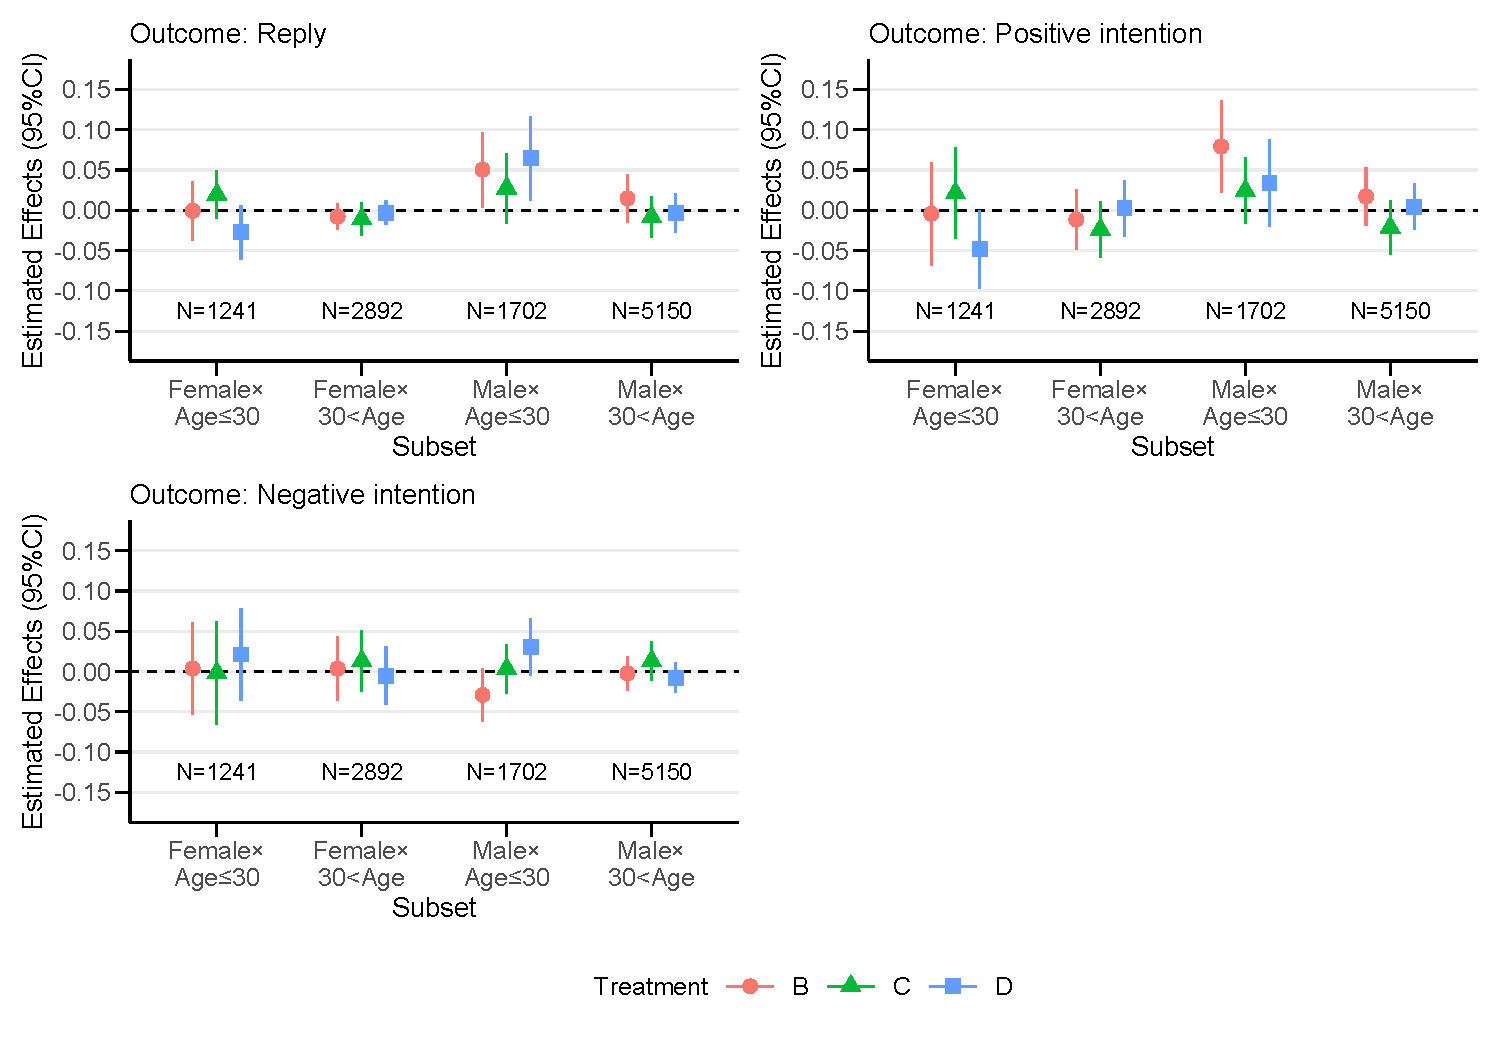
\includegraphics[width=0.75\linewidth]{C:/Users/vge00/Desktop/JMDP/RCT-Nudge/docs/slide/221024骨髄バンク介入実験分析_files/figure-beamer/plot-reg-stock-by-genage-1} \end{center}
\end{frame}

\begin{frame}{フロー変数(返信日数)の分析}
\protect\hypertarget{ux30d5ux30edux30fcux5909ux6570ux8fd4ux4fe1ux65e5ux6570ux306eux5206ux6790}{}
\begin{itemize}
\tightlist
\item
  適合通知を送付してから\(X\)日以内に返信したかどうか(提供を希望して返信したかどうか/提供を希望しないで返信したかどうか)をアウトカム変数として、効果の経時的変化を分析する

  \begin{itemize}
  \tightlist
  \item
    適合通知には、\textbf{7日以内}の返信をお願いしている
  \end{itemize}
\end{itemize}
\end{frame}

\begin{frame}{返信日数の分布}
\protect\hypertarget{ux8fd4ux4fe1ux65e5ux6570ux306eux5206ux5e03}{}
\begin{center}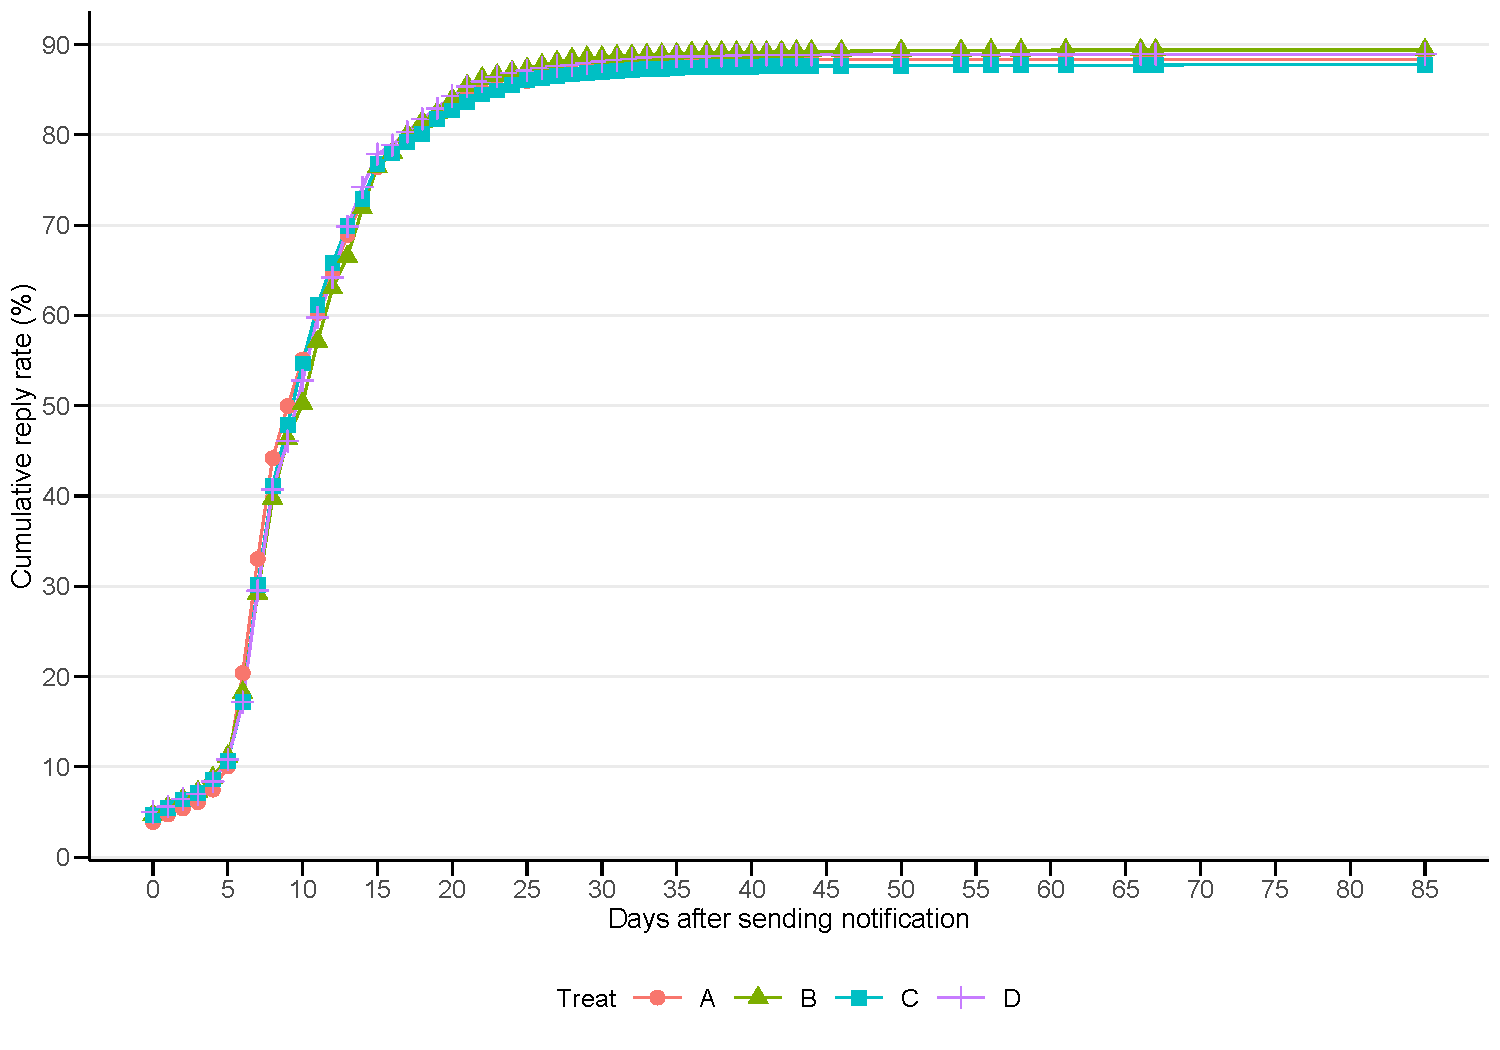
\includegraphics[width=0.75\linewidth]{C:/Users/vge00/Desktop/JMDP/RCT-Nudge/docs/slide/221024骨髄バンク介入実験分析_files/figure-beamer/dist-days-reply-1} \end{center}
\end{frame}

\begin{frame}{フルサンプルの分析結果}
\protect\hypertarget{ux30d5ux30ebux30b5ux30f3ux30d7ux30ebux306eux5206ux6790ux7d50ux679c}{}
\begin{center}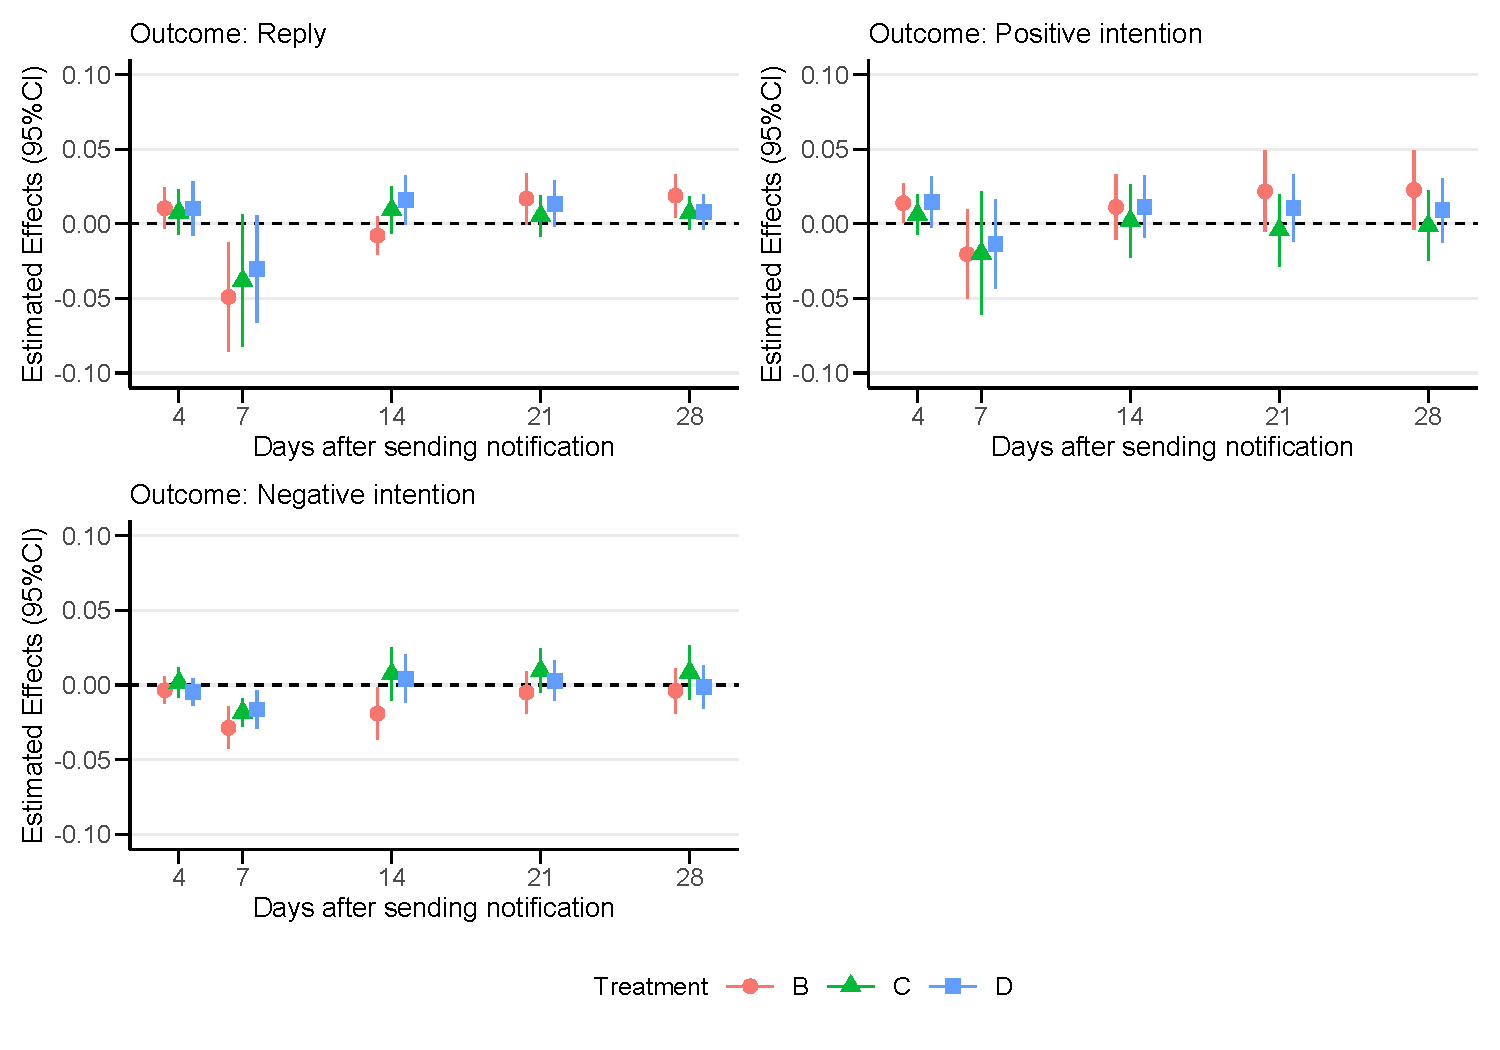
\includegraphics[width=0.75\linewidth]{C:/Users/vge00/Desktop/JMDP/RCT-Nudge/docs/slide/221024骨髄バンク介入実験分析_files/figure-beamer/plot-reg-flow-1} \end{center}
\end{frame}

\begin{frame}{異質性:30歳以下の女性}
\protect\hypertarget{ux7570ux8ceaux602730ux6b73ux4ee5ux4e0bux306eux5973ux6027}{}
\begin{center}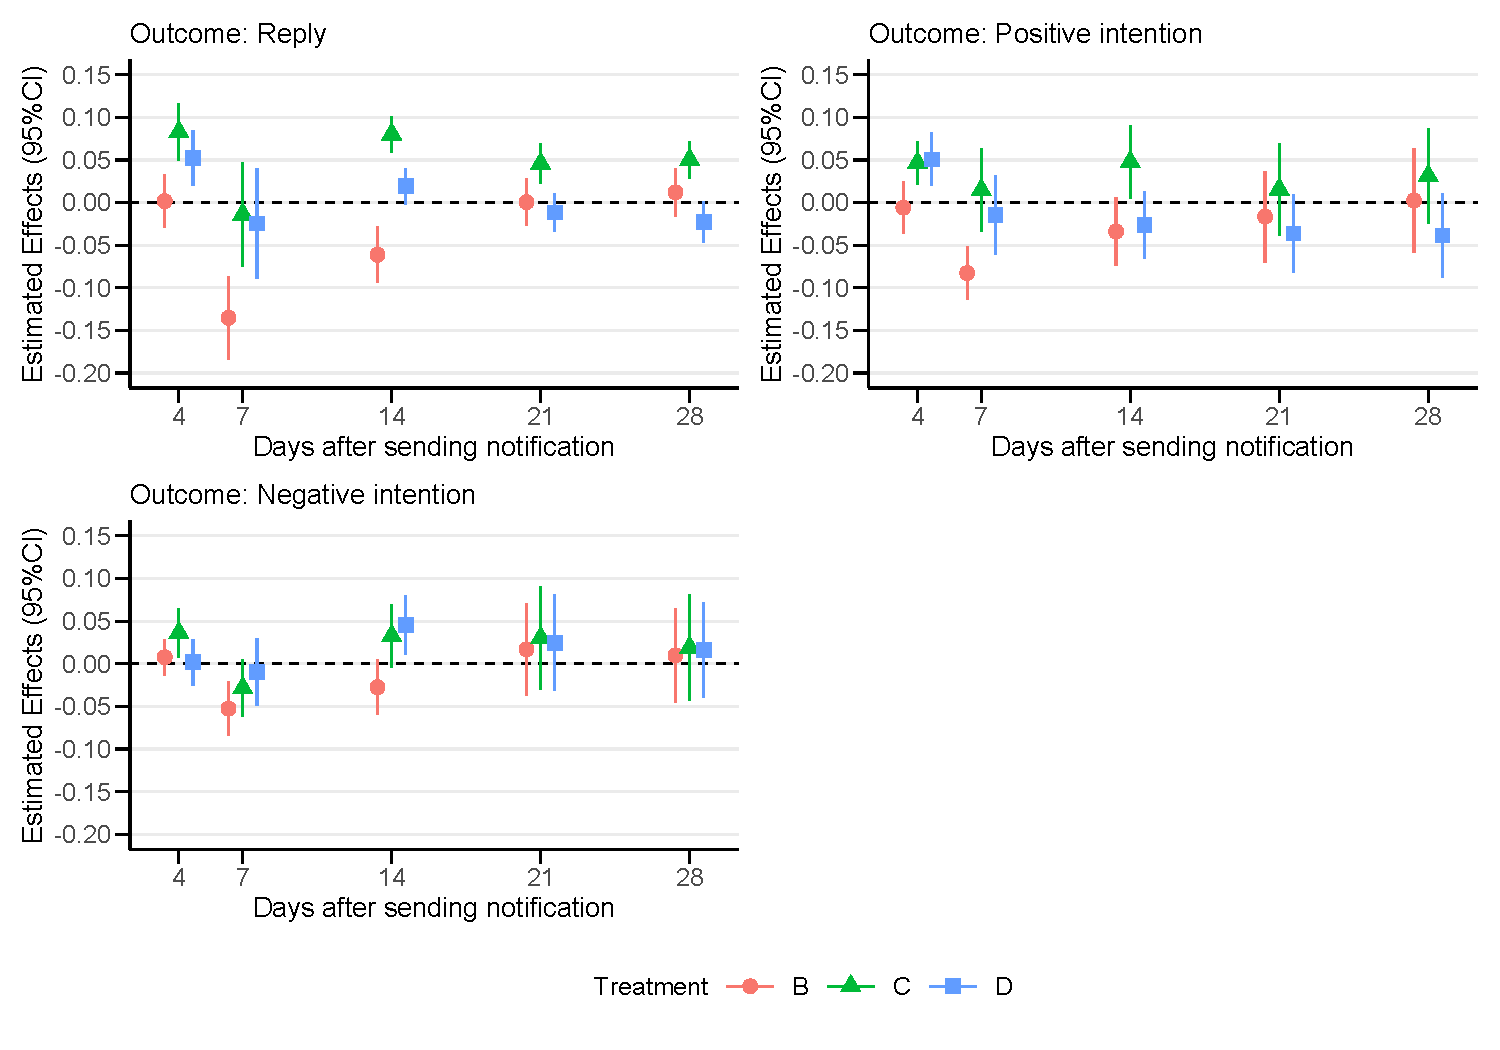
\includegraphics[width=0.75\linewidth]{C:/Users/vge00/Desktop/JMDP/RCT-Nudge/docs/slide/221024骨髄バンク介入実験分析_files/figure-beamer/plot-reg-flow-female-less30-1} \end{center}
\end{frame}

\begin{frame}{異質性:30歳を上回る女性}
\protect\hypertarget{ux7570ux8ceaux602730ux6b73ux3092ux4e0aux56deux308bux5973ux6027}{}
\begin{center}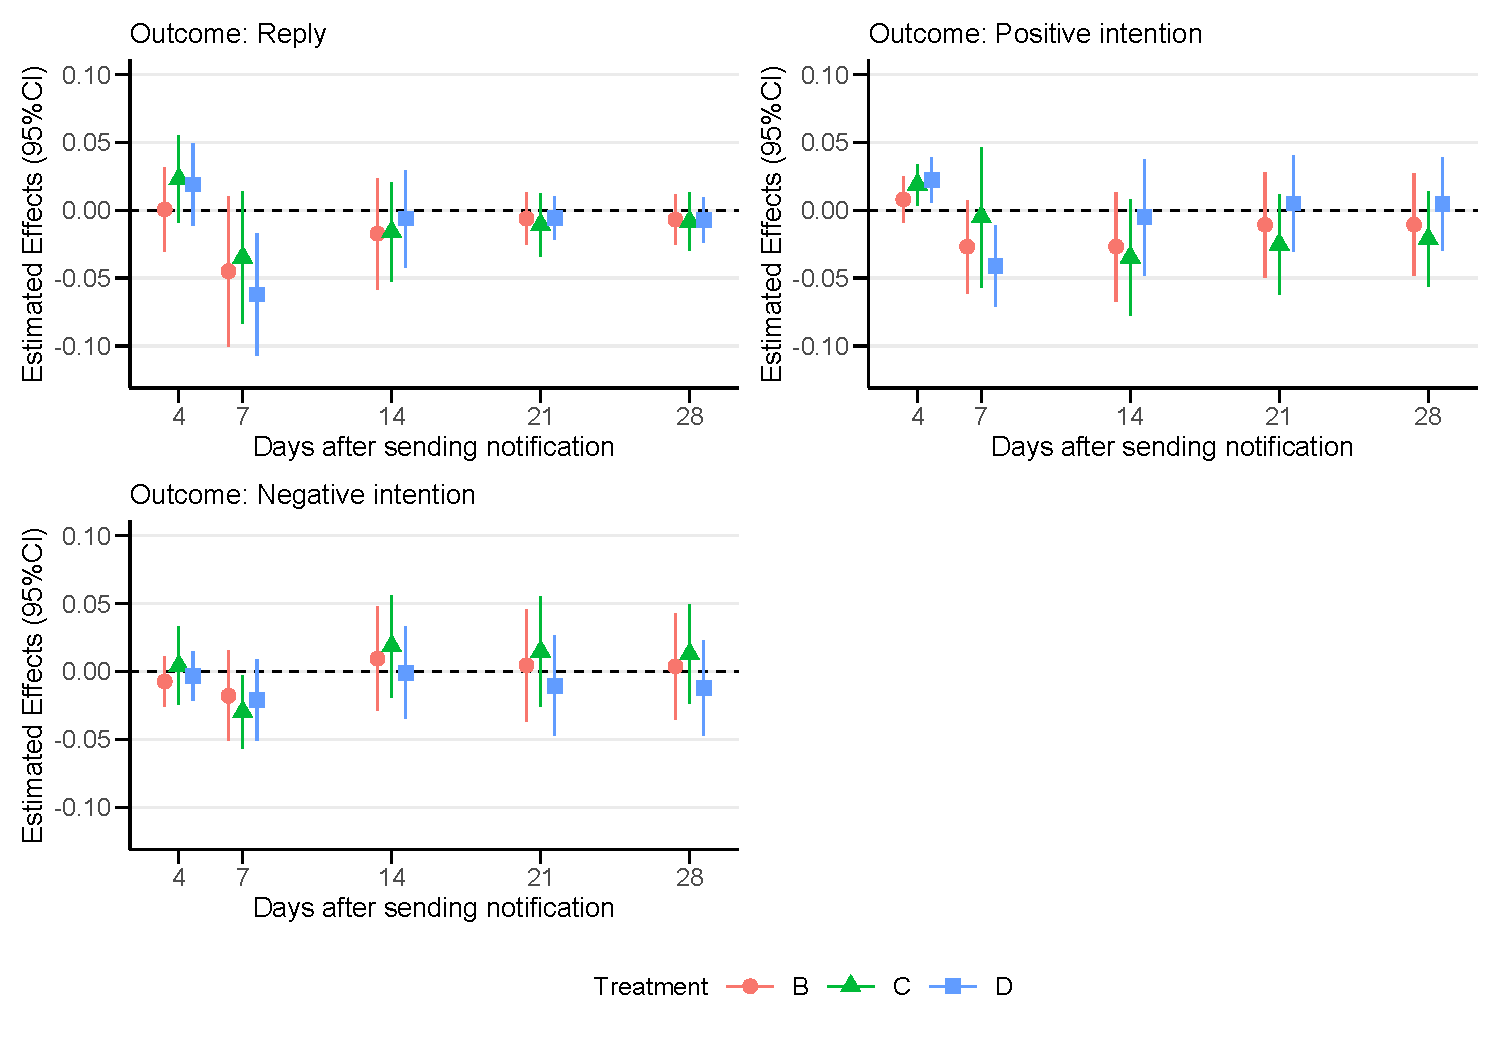
\includegraphics[width=0.75\linewidth]{C:/Users/vge00/Desktop/JMDP/RCT-Nudge/docs/slide/221024骨髄バンク介入実験分析_files/figure-beamer/plot-reg-flow-female-over30-1} \end{center}
\end{frame}

\begin{frame}{異質性:30歳以下の男性}
\protect\hypertarget{ux7570ux8ceaux602730ux6b73ux4ee5ux4e0bux306eux7537ux6027}{}
\begin{center}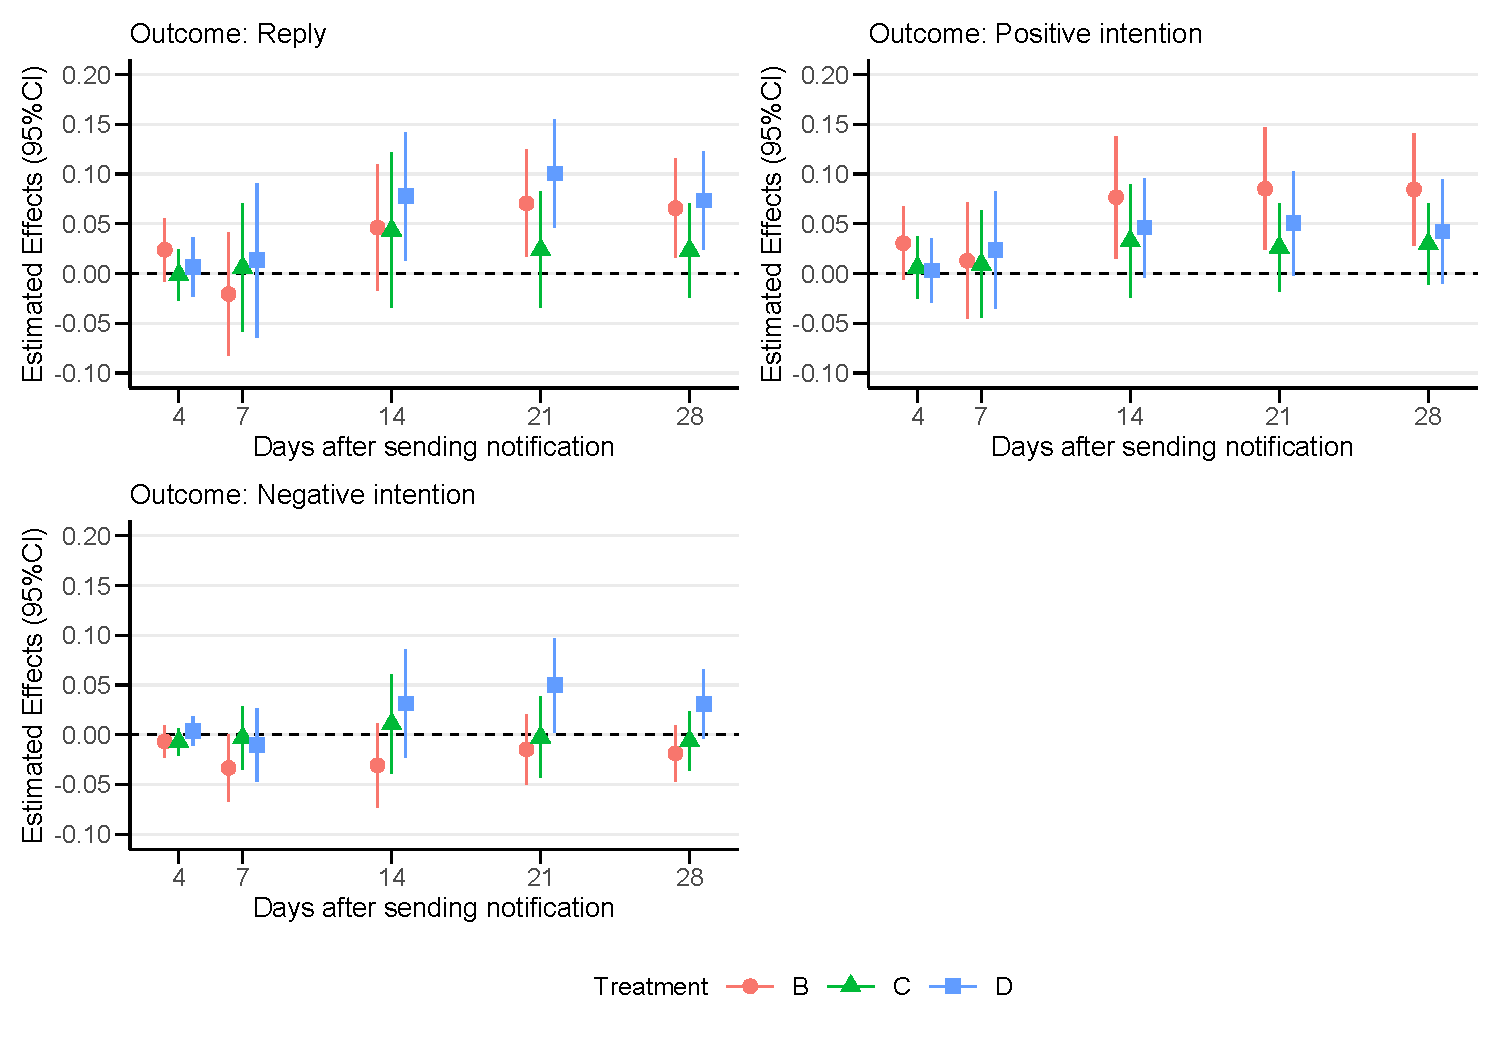
\includegraphics[width=0.75\linewidth]{C:/Users/vge00/Desktop/JMDP/RCT-Nudge/docs/slide/221024骨髄バンク介入実験分析_files/figure-beamer/plot-reg-flow-male-less30-1} \end{center}
\end{frame}

\begin{frame}{異質性:30歳を上回る男性}
\protect\hypertarget{ux7570ux8ceaux602730ux6b73ux3092ux4e0aux56deux308bux7537ux6027}{}
\begin{center}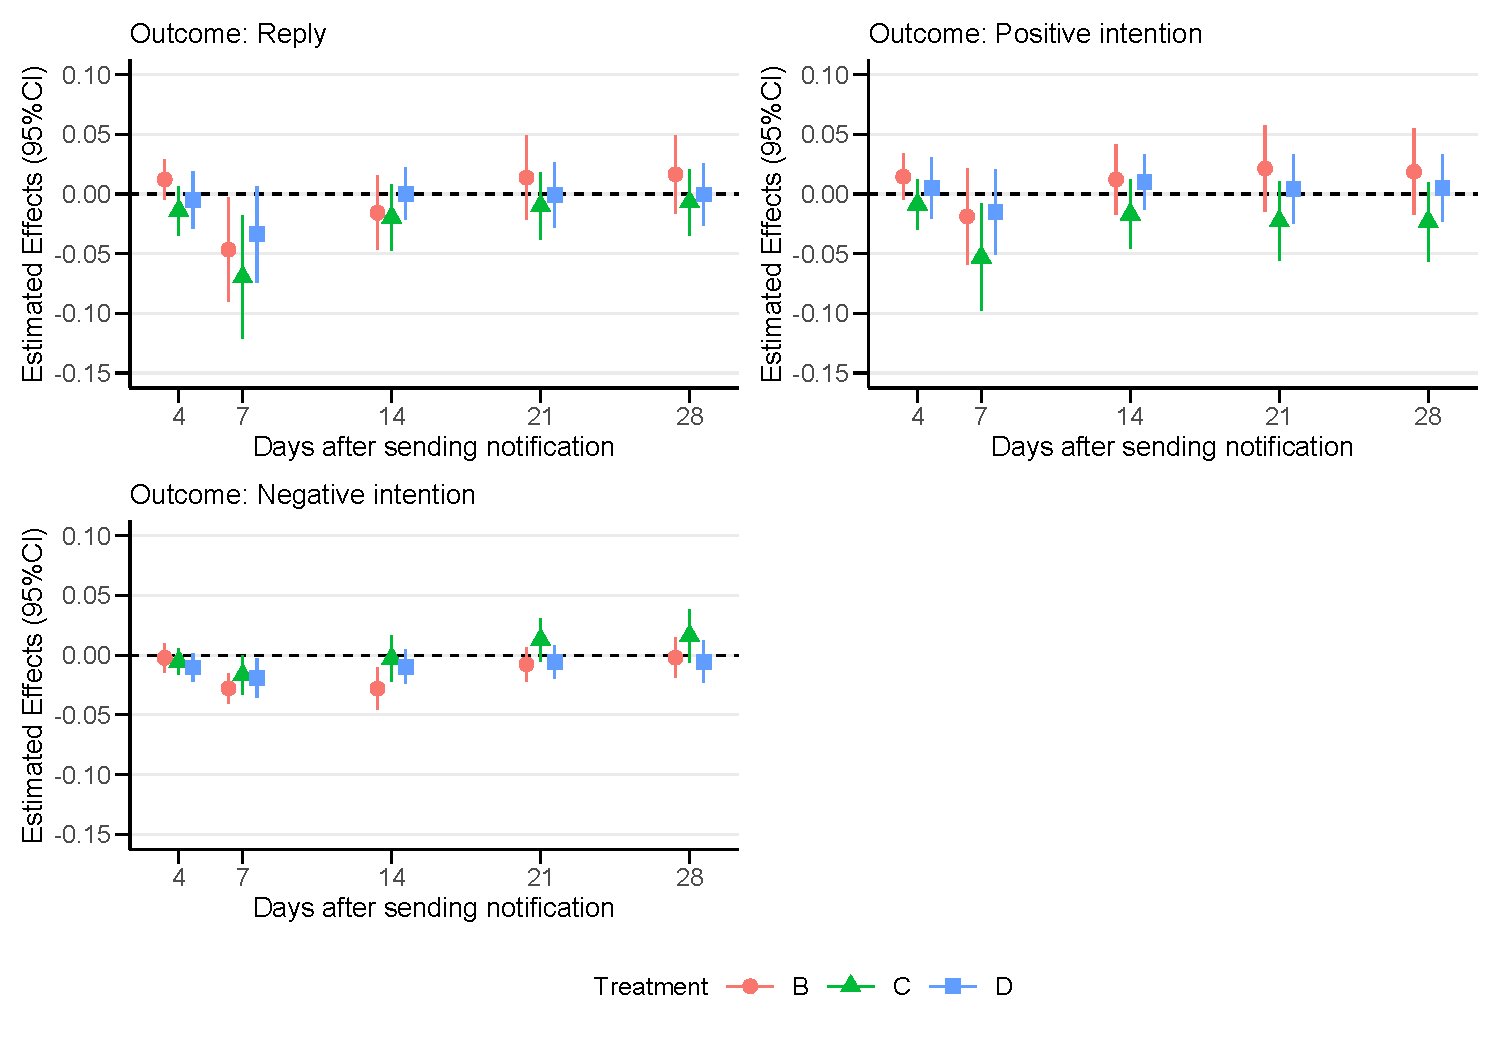
\includegraphics[width=0.75\linewidth]{C:/Users/vge00/Desktop/JMDP/RCT-Nudge/docs/slide/221024骨髄バンク介入実験分析_files/figure-beamer/plot-reg-flow-male-over30-1} \end{center}
\end{frame}

\begin{frame}{地域による異質性の検討}
\protect\hypertarget{ux5730ux57dfux306bux3088ux308bux7570ux8ceaux6027ux306eux691cux8a0e}{}
\begin{itemize}
\tightlist
\item
  メッセージBは面談施設が多い都道府県(東京・大阪・愛知・神奈川)に在住している人に対しても有効
\item
  性別×地域による異質性を分析すると、メッセージBは面談施設が多い地域に住む女性に対して有効ではないが、
  面談施設が多い地域に住む男性に対して有効である。
\end{itemize}
\end{frame}

\hypertarget{appendix-a.-heterogeneity-by-region}{%
\section{Appendix A. Heterogeneity by Region}\label{appendix-a.-heterogeneity-by-region}}

\end{document}
